\chapter{Quantum-dot cellular automata}
\graphicspath{{../gfx/chapter01/}}


\section{The idea}

\begin{figure}
  \center
  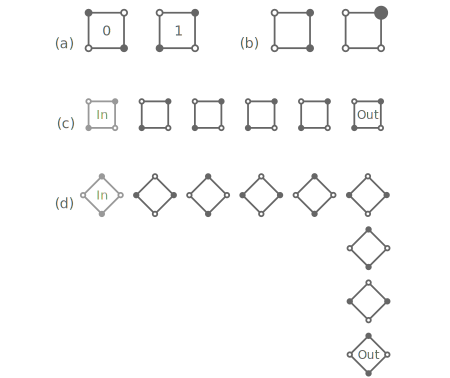
\includegraphics{intro_qca}
  \caption{
Building blocks of quantum-dot cellular automata (QCA). (a) A QCA cell consists
of four quantum dots on the corners of a square and is occupied by two
electrons. Due to Coulomb repulsion two energetically preferred states emerge,
logic 0 and logic 1. (b) Both electrons occupying the edge of the cell or
doubly occupying a single quantum dot are unfavourable high-energy states. (c) A
straight line of cells functions as a wire and transmits a signal.  (d) A
diagonal line of cells (cells rotated by $45^{\circ}$) transmits a signal
alternating from cell to cell. Wires can have kinks.
}
  \label{fig:intro_qca}
\end{figure}
%
\begin{figure}
  \center
  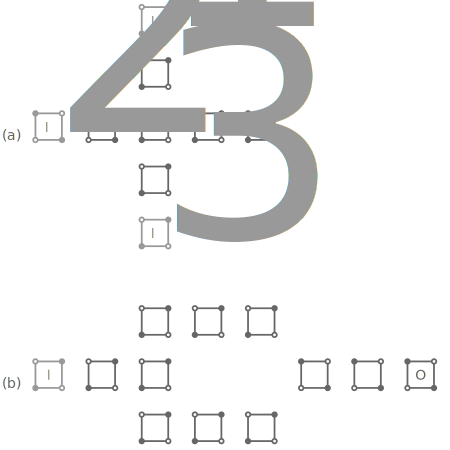
\includegraphics{gates}
  \caption{
QCA gates. (a) The majority gate's three inputs ``vote'' on the output. The gate
is commonly operated with one fixed input, for example $I_3$, and then functions
as an AND ($I_3 = 1$) or OR gate ($I_3 = 0$) for the remaining two inputs. Here
the gate performs the computation $1 \land 0 = 1$. (b) The inverter inverts a
signal.
}
  \label{fig:gates}
\end{figure}

Lent et al.\ introduced the concept of quantum-dot cellular automata as an
alternative computing paradigm in 1993 \cite{lent1993quantum}. The aim was a
novel physical scheme to build digital circuits that would overcome some of the
limitations of CMOS technology, promising potentially lower power consumption,
higher device density, and faster clocking. As the name alludes to, quantum-dot
cellular automata (QCA) is made from quantum dots which are grouped into cells.
Figure~\ref{fig:intro_qca}(a) shows a basic QCA cell. Four quantum dots are
arranged on the corners of a square. The dots are idealized as perfectly
localized single orbitals on a perfectly decoupled non-intrusive medium.
Therefore, each dot can be occupied by up to two electrons. In the QCA scheme,
however, each cell is occupied by only two electrons in total, the cell is
quarter-filled. The electrons tunnel between different dots in a cell, but the
dominant energy scale has to be the Coulomb repulsion between the particles.
Simply by virtue of the Coulomb repulsion, and ignoring the assumedly
comparatively small tunnelling for now, the diagonal states are the two
energetically preferred electron configurations as indicated in the figure. In
comparison, edge states or doubly occupied quantum dots are unfavourable higher
energy states, Figure~\ref{fig:intro_qca}(b). A priori the two diagonal states are
energetically degenerate, but this degeneracy can be lifted by an external
Coulomb potential, for example a second nearby QCA cell. Then these two states
can be identified with logic 0 and 1, respectively.

A single cell by itself is not very interesting. But multiple cells can be
positioned next to each other, for example as a straight line of cells,
Figure\ref{fig:intro_qca}(c). The approach now again assumes that Coulomb is the
driving force and that electron tunnelling between cells is very small and
ideally zero. For a straight line of cells, the long-ranging, unscreened Coulomb
forces will tend to align the electron configurations of adjacent cells.  If the
first cell is in logic state 1 then the second cell will also prefer logic state
1 and so will in turn all the other cells in the line. The situation is the same
for logic state 0. Therefore, a straight line of cells is similar to a wire not
only in geometry, but also in functionality: It transmits a digital signal. The
same is true, with slight modifications, for a diagonal line of cells---cells
rotated by $45^{\circ}$, Figure~\ref{fig:intro_qca}(d). In this case the signal
alternates from cell to cell, that is, logic 1 will follow logic 0 which
followed from logic 0, and this again is simply by virtue of the dominant
Coulomb interaction between electrons on different cells. By using an even
number of cells the diagonal line of cells works as a wire just as well as a
straight line of cells. The pictogram also demonstrates a $90^{\circ}$ kink for
the diagonal line of cells which our newly gained intuition for these
Coulomb-driven systems expects to pose no problem for signal transmission.

The main idea of the QCA approach becomes apparent: Ideally bistable cells
interact with each other solely by Coulomb repulsion. By arranging the cells in
clever geometries we can realize interesting functionalities. The idea as such
is quite general and does not strictly rely on the two-electron-four-dot cell
introduced above. Indeed, a number of variations exist, such as cells consisting
of only two dots and occupied by only one electron, interacting via dipole
fields instead of quadrupole fields as for the conventional cells. Another
variation is a four-dot cell with six electrons---two holes---instead of two
electrons. Even the interaction need not be Coulombic. For example, magnetic QCA
schemes have been explored. While QCA carries ``quantum'' in its name and is
sought to be implemented at the nanoscale, the approach operates close to the
classical limit. The Coulomb interaction is absolutely dominating with the
tunnelling of electrons a small perturbation, which nonetheless drives the
system's dynamics.  The approach is insensitive and in fact ignores the spin
degree of freedom. Let us finally note that QCA is a not a cellular automata in
a strict mathematical sense, but only by analogy to the idea of interacting
cells.

One clever geometrical cell arrangement is shown in Figure~\ref{fig:gates}(a),
the majority gate. The gate has three inputs which ``vote'' on the central cell.
The majority wins and sets the single output. The device is commonly operated
with one fixed input, for example $I_3 \doteq 0$ or $I_3 \doteq 1$. In the first
case, $I_3 \doteq 0$, the device functions as an AND gate for the remaining two
inputs, $O = I_1 \land I_2$. In the second case, $I_3 \doteq 1$, it is an OR
gate with $O = I_1 \lor I_2$. The figure shows the gate performing the
computation $1 \land 0 = 1$. Now, the only missing piece for Boolean algebra is
negation, $O = \lnot I$. We had already seen that simply arranging cells at an
$45^{\circ}$ angle as in the diagonal line of cells negates the signal from cell
to cell. The inverter, Figure~\ref{fig:gates}(b), recasts this idea into a more
robust layout. With that we have, at least in principle, all the necessary
building blocks for Boolean algebra and thus digital circuitry.

Conceptually, it is most elegant to set the inputs for a QCA circuit via driver
cells---cells that resemble the QCA cell in form, but are made up from static
point charges instead of quantum dots. These static charges are thought to be
manipulatable to vary the input smoothly from the logic 0 to the logic 1 state.
In Figures~\ref{fig:intro_qca}~and~\ref{fig:gates} these driver cells are
represented in light grey.  Of course, in practice such driver cells would be
difficult if not impossible to implement and the inputs are more likely set by
leads that provide the necessary perturbative electrostatic fields. The output
of a QCA device can be directly read from its output cells. In practical
implementations this will require a non-trivial charge probing apparatus.
Changing the input for a QCA device throws the system into an excited,
non-equilibrium state. The system will then dissipatively propagate to its new
ground state. For the given inputs, this ground state corresponds to the
solution of the computational problem the circuit is designed to solve. Let us
emphasize this: In QCA, the computational solution maps directly to the physical
ground state. During performing a computation only a few charges move locally,
in each cell. Operating close to the ground state, QCA is thus a truly
current-free approach and consequently inherently low-power, especially when
compared with CMOS technology. But the operation close to the ground state also
raises concerns for the operational temperature for these devices. It is clear
that for applications we would want to engineer the system so that the energy
gap between the ground state and the low-lying excited states far exceeds room
temperature.  Different material systems provide different dissipative channels
and modelling them quantitatively or even qualitatively correctly is very
challenging. As a consequence, it is difficult to derive general expectations
for the clocking speed of QCA circuits.  The switching speed of a majority gate,
for example, will greatly depend on the system's parameters, but particularly on
the nature of the dissipative coupling of the circuit to its environment. A
small dissipative coupling will have the output polarization oscillating before
it eventually settles to its correct value. A very dissipative system in
contrast might get stuck in meta-stable states. 

QCA circuits consist of wires, gates, and other structures arranged on a
two-dimensional surface---very similar to conventional electronics devices.
However, the structures themselves are quasi-one-dimensional and this poses a
challenge for building large-scale QCA circuits. A good example is a single long
wire, which is truly one-dimensional. When we think about switching the input
for the wire, we think of the information being propagated as a charge density
wave throughout the line of cells, or, equivalently, as propagating the domain
boundary between logic 0 and logic 1. This domain boundary incurs an energy cost
that the system seeks to minimize, causing the wire to order. For an
increasingly longer wire, however, the gain in entropy for moving a domain
boundary freely throughout the wire ($S \sim \log N$, $N$ the number of cells)
soon exceeds the loss in energy, which is reflected by the free energy of the
system ($F = U - T S$). Quite generally, a one-dimensional system cannot be
ordered in the thermodynamic limit except at zero temperature. Therefore, the
finite-temperature infinitely long wire will always have at least two different
domains, logic 0 and logic 1, and thus not be able to transmit a signal. The gap
between the first excited state---with two domains---and the completely ordered
ground state, together with the desired operational temperature will determine
the maximum system size.
% TODO: would be nice to have a reference for the fact that 1D systems cannot be
% ordered

\begin{figure}
  \center
  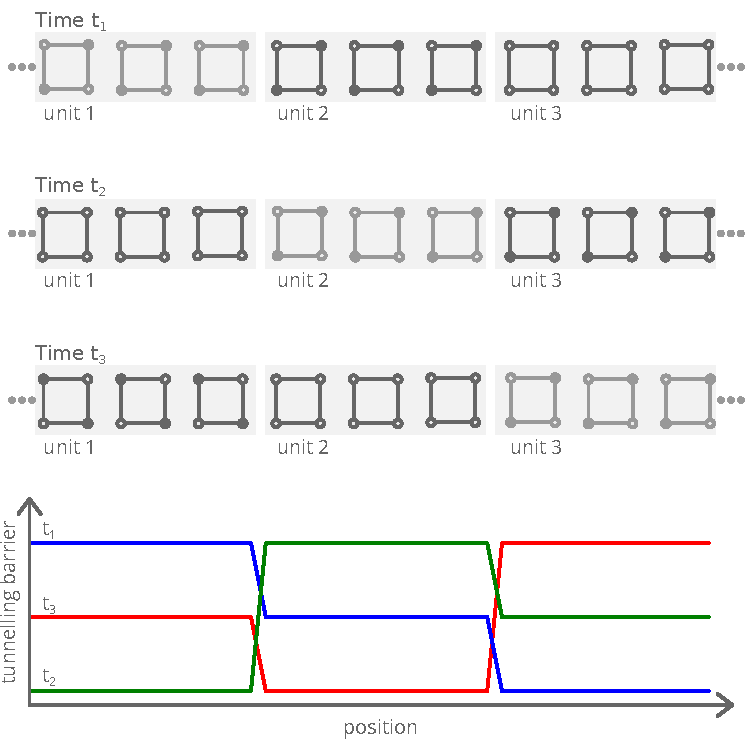
\includegraphics{clocking}
  \caption{
Clocked QCA for a line of cells. To avoid entropy-induced disorder in large QCA
circuits, the system is partitioned into smaller units: unit 1, 2, and 3 in this
example. By varying the tunnelling barriers, each unit is put through the three
phases \emph{frozen} (high barrier, light grey cells), \emph{active} (medium
barrier, dark grey cells), and \emph{delocalized} (low barrier, dark grey cells
with empty dots). Synchronizing the phases of adjacent units allows to pipeline
information flow and computations.  The line of cell's three units and their
tunnelling barriers are shown at three different times, $t_1<t_2<t_3$. A logic 1
state is propagated from the left to the right.  At $t_3$ a logic 0 state is
coming in from the left.
}
  \label{fig:clocking}
\end{figure}

To address this scaling problem we partition large circuits into smaller units.
The size of each unit is chosen to be small enough to avoid entropy-induced
disorder at a given operational temperature. Each unit can be turned ``on'' and
``off'' separately: Ideally, individual gates would allow to effectively raise
and lower the tunnelling barriers between quantum dots in each unit and thus
allow to freeze or delocalize the electrons. A unit with \emph{frozen} electrons
can serve as the input for a unit with more \emph{active} charge carriers, which
works like a regular QCA circuit. A unit with completely \emph{delocalized}
electrons, in contrast, will not influence adjacent units. By putting each unit
through the three phases \emph{delocalized}, \emph{active}, and \emph{frozen}
and synchronizing adjacent units appropriately, we can control the information
flow through the system very nicely, as illustrated in Figure~\ref{fig:clocking}.
Therefore, by partition the circuit and introducing a clocking scheme we not
only handle the scaling problem, but also arrive at a pipelining architecture.
If and how the tunnelling barriers can be effectively modified will depend on
the details of the specific QCA implementation. Also, in practice the QCA
circuit units cannot be too small as they must be individually addressable.
Gates which turn QCA units ``on'' and ``off'' provide another potential benefit
as well. We are able to control how and especially how fast the gate voltage is
changed and should be able to tune it with respect to the inherent time-scales
of the QCA system, which are set by the system's parameters and the dissipative
coupling to its environment. This should afford a better control over the
dynamics of the switching process and might help mitigate problems like
oscillating outputs and meta-stable states, mentioned above
\cite{lent1997device}.
% TODO: clarify how the raising and lowering of the tunnelling barriers could
% really plausibly work, e.g. for the silicon system


\section{Atomic silicon quantum dots}

\begin{figure}
  \center
  \includegraphics{silicon}
  \caption{
Atomic silicon quantum dots are \emph{dangling bonds} (DBs) on a hydrogenated
(100) silicon surface. (a) A scanning tunnelling microscope (STM) image of an
atomic silicon quantum dot QCA cell. (b) Band diagram of a DB on a strongly
n-doped silicon substrate. (c) The reconstructed (100) hydrogenated silicon
surface, showing dimer rows. (d) Two closely spaced tunnel-coupled DBs perturbed
by a third DB (bottom left). All STM images and \emph{ab initio} estimates from
Wolkow et~al.\ \cite{wolkow2013silicon} \cite{pitters2011tunnel}.
}
  \label{fig:silicon}
\end{figure}

Our objective is the general, not implementation-specific characterization of
the QCA approach. Even so it is still important to consider concrete
experimental realizations, not only as a motivation for our work, but also to
put our modelling and results into context. One of the most promising and recent
experimental implementations of QCA is based on atomic silicon quantum dots and
we will therefore use them as our experimental reference. Atomic silicon quantum
dots were first demonstrated as a possible QCA implementation by Wolkow et~al.\
in 2009, when the group realized one single QCA cell.
Figure~\ref{fig:silicon}(a) shows a scanning tunnelling microscope (STM) image
of this cell. Since then impressive advances have been made both in the
understanding of the electronic properties of these quantum dots as well as in
the precise fabrication of larger QCA structures. With atomic-scale feature
sizes this experimental system promises room temperature operation, while at the
same time tapping into the established and highly-sophisticated silicon
technology. Being based on silicon should also ease integration with existing
CMOS circuitry.

Atomic silicon quantum dots are \emph{dangling bonds} on a hydrogen-terminated
$(100)$ silicon surface. Atoms on a $(100)$ silicon surface have two unsatisfied
bonds. Pairs of surface atoms form dimers, satisfying one bond. The remaining
bond is satisfied by passivating the surface with hydrogen.
Figure~\ref{fig:silicon}(c) shows a STM image of the reconstructed silicon
surface, where the dimer rows are clearly visible and the dimensions are
indicated. By applying a relatively large current through the STM tip,
individual hydrogen atoms can be removed, with atomic precision. This leaves a
\emph{dangling bond} (DB) which acts as a quantum dot: Energetically, electrons
on the DB orbital sit in the silicon band gap and are therefore decoupled from
the silicon substrate.  Figure~\ref{fig:silicon}(b) shows the band diagram of a
DB on a n-doped substrate.  Chemically, DBs have proven to be surprisingly
robust with respect to environmental molecules. From \emph{ab initio}
calculations it is known that the $sp^3$ DB orbital extends predominantly into
the bulk and only a little into the vacuum. The orbital's lateral extent is on
the order of $1\mathrm{nm}$ and therefore spans multiple silicon lattice atoms.
Due to orbital overlap, closely spaced DBs are tunnel-coupled. A neutral DB
consists of the positive silicon ion and one electron. In the experimentally
common strongly n-doped system, the DB accepts one more electron and is
therefore $-1e$ negatively charged. Conversely, in a p-doped sytem the DB will
donate its electron and become $+1e$ positively charged. The Coulomb repulsion
between negatively charged DBs can be used to adjust the filling of DB
assemblies simply by the DBs' positions. For example, on a n-doped substrate two
DBs may eject one electron (which goes back to the bulk) and share the remaining
single electron, when placed close enough together. To proof this, a third DB is
placed close by, but not close enough to be tunnel-coupled. The effect of the
Coulomb repulsion can be seen via STM imaging, Figure~\ref{fig:silicon}(d),
where the DB farthest from the perturbing external charge is more negatively
charged (darker in the STM image) than the closer DB. The observed charge shift
is only possible when both closely-spaced DBs share a single electron. To form
the previously shown QCA cell, Figure~\ref{fig:silicon}(a), on a strongly
n-doped silicon substrate four DBs are brought close enough together so that two
electrons go back to the bulk, leaving the cell with six electrons (two holes)
in total and a cell net charge of $-2e$---the right charge regime for QCA.

Atomic silicon quantum dots provide some examples of how a real world system
might be different from the idealized picture we typically employ to describe
the QCA approach. We like to think of quantum dots as perfectly localized
orbitals. But in the silicon system the orbitals of the DBs actually span
multiple lattice sites and only if the DBs are placed far enough apart, might we
still be able to consider them as localized. We do not consider the substrate
but treat quantum dots as perfectly isolated entities. Of course, in practice
the substrate will certainly influence the QCA device. In the silicon system
free charge carriers will screen the long-ranged Coulomb interactions that the
QCA scheme relies on. The screening is not necessarily disruptive for QCA and
might even be beneficial, for example by minimizing charge-buildup in large
systems. But to quantify the screening effect accurately, thorough understanding
and precise modelling are necessary, which, for atomic silicon quantum dots
which live at the surface, would surely be very challenging. The silicon
substrate could also, conceivable, provide a second tunnelling channel between
DBs. In addition to electrons hopping directly from DB to DB they could first
tunnel from the first DB to the substrate and then back to the second DB. Thus
an accurate model for atomic silicon quantum dots might need to accommodate the
nature of the DB orbitals, screening, multiple tunnelling channels and other
effects.


\section{The extended Hubbard model}

QCA systems are typically modelled by an extended Hubbard Hamiltonian. The
Hubbard model originated in the early 1960s to describe rare-earth systems with
highly localized d- and f-electrons and has since then, of course, become one of
the most widely studied and successful models in condensed matter physics
\cite{Hubbard1964}. In basing our description on the Hubbard model we already
put some key assumptions in place. For example, we assume that the quantum dots
are similar to the highly localized d-orbitals. As discussed above, depending on
the particular QCA implementation this might or might not be a good description.
However, our interest is not in the precise details of any particular material
system QCA might be implemented on, but our aim is to investigate universal
characteristics of QCA systems. An idealized but semi-realistic description is
what we want and for that the Hubbard model is indeed an appropriate---and
tractable---starting point. Specifically, the Hamiltonian we use is
\begin{equation}
  \label{eq:H_QCA}
  H =
    - \sum_{ij\sigma} t_{ij} \, c^{\dagger}_{i\sigma} c_{j\sigma}
    + U \sum_i n_{i\uparrow} n_{i\downarrow}
    - \mu \sum_{i\sigma} n_{i\sigma}
    + \sum_{i<j} V_{ij} \left( n_{i\uparrow} + n_{i\downarrow} - q \right) 
                        \left( n_{j\uparrow} + n_{j\downarrow} - q \right) \, ,
\end{equation}
where $c^{\dagger}_{i\sigma}$ ($c_{i\sigma}$) creates (annihilates) an electron
on quantum-dot $i$ with spin $\sigma$ and the particle number operator is
$n_{i\sigma} = c^{\dagger}_{i\sigma} c_{i\sigma}$; $t_{ij}$ is the overlap integral between
dots $i$ and $j$, $U$ is the Hubbard on-site Coulomb repulsion, $\mu$ the
chemical potential, and $V_{ij}$ the long-ranged Coulomb interaction, which is
characteristic for QCA systems. For simplicity the Coulomb term is chosen to be
$V_{ij} = \frac{1}{r_{ij}}$ where $r_{ij}$ is the distance between the two dots
$i$ and $j$. We also introduce the \emph{compensation charge} $q$ which is
thought to represent a possible positive ion at each quantum dot site. This
constant positive charge allows us to tune the net cell charge. For two
electrons per cell, for example, $q=0$ yields a net cell charge of $-2e$ whereas
$q = \frac{1}{2}$ represents zero net cell charge, and here the cell becomes a
perfect electrostatic quadrupole.

The geometric layout of the QCA system and therefore its functionality is
encoded in the hopping parameter $t_{ij}$ and the long-ranged Coulomb term
$V_{ij}$. For the hopping parameter we usually only consider nearest-neighbour
hopping $t$ and specifically no hopping between the cells. While this constraint is
not strictly necessary for QCA, it is in line with the approach's underlying
idea and greatly simplifies calculations. Because the overlap integral decays
exponentially with distance, as long as the distance between dots from different
cells is larger then the distance between dots within one cell, the assumption will
introduce only a small error. Still, this is something to keep in mind if we
place cells very close to each other. Note that without inter-cell hopping we can
decompose the Hamiltonian into purely Coulombic cell-cell interaction terms
$H^{cc}_{kl}$ and single cell terms $H^c_k$ which capture the kinetics as well
as the inside-cell Coulomb interactions,
\begin{equation}
  \label{eq:H_cell}
  H = - \sum_k H^c_k + \sum_{k<l} H^{cc}_{kl} \, ,
\end{equation}
where $k$ and $l$ number the cells. 

\begin{figure}
  \center
  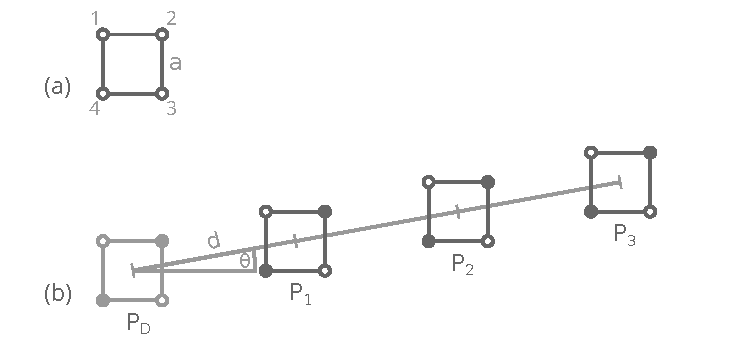
\includegraphics{short_wire}
  \caption{\ldots}
  \label{fig:short_wire}
\end{figure}

To parameterize the Coulomb term $V_{kl}$ and specifically $r_{ij}$, the
distance between quantum-dots $i$ and $j$, we introduce the cell edge length $a$
and the cell-cell distance $d$, as illustrated in Fig.~\ref{fig:short_wire}
where we have used a short line of cells as an example QCA system. The angle
between adjacent cells is denoted by $\theta$. Ideally each cell should be in
logic state 0 or logic state 1, but, of course, in practice a cell can be in any
superposition of the two states or even in a different state altogether. The
\emph{cell polarization} $P_k$ quantifies the state of the cell,
\begin{equation}
  \label{eq:polarization}
  P_k = \frac{1}{2} \left( n_{4k+2} + n_{4k+4} - n_{4k-1} + n_{4k-3} \right) \, ,
\end{equation}
where the dots in each cell are numbered clockwise as indicated in the figure
and we have introduced the shorthand notation $n_i = n_{i\uparrow} +
n_{i\downarrow}$. The cell polarization is $P_k = -1$ for a logic 0 and $P_k =
+1$ for a logic 1 state. Without any external input the polarization of a cell
will be $P_k = 0$.  In the example line of cells, the input is set via the
driver cell's polarization $P_D$ at the left end. The driver cell's four static
point charges are adjusted to reflect the desired polarization $P_D$. For QCA,
the cell polarization really is the observable of utmost interest. It indicates
whether a cell is in logic state 0 or logic state 1 and how polarized the cell
is, where ideally, of course, the cell should always be fully polarized $|P_k| =
1$. In short, the cell polarizations will indicate how well the QCA approach
works for a given system and, unsurprisingly, calculating cell polarizations for
various geometric layouts over a wide range of system parameters will be our
main focus.

The QCA cell is characterized by three energy scales: the nearest-neighbour
hopping $t$, the nearest-neighbour Coulomb repulsion $V_1 = \frac{1}{a}$, and
the on-site Coulomb repulsion $U$. For QCA operation $U$ is usually assumed to
be sufficiently large so that doubly occupied states are gapped out. We can
introduce $V_2 = \frac{1}{\sqrt{2} a}$, the next-nearest-neighbour Coulomb
repulsion, which corresponds to both electrons sitting on the diagonal of the
cell---our preferred $P=\pm1$ states, ideally the ground state. Conversely,
$V_1$ corresponds to both electrons occupying the edge of the cell. Again, for
QCA operation we would like the edge states to be sufficiently gapped out.
Therefore, the energy gap $\Delta V = V_1 - V_2 = \frac{2 - \sqrt{2}}{2 a} \sim
0.3 V_1$ and to a lesser extent $U \gg \Delta V$ will directly determine how
polarized our cell is. $V_1$ will thus seek to order the cell. It competes with
the hopping $t$ which delocalizes and unorders the electrons. QCA is thought to
function in a regime where the ratio $\frac{V_1}{t}$ is large. Of course, it is
also clear that if $\frac{V_1}{t}$ becomes too large, for example by taking $t
\rightarrow 0$, the system becomes slower and eventually freezes which is also
undesirable for QCA operation. To complete the picture we have to put in the
temperature $T$, because what we really mean by saying ``sufficiently gapped
out'' is an energy gap relatively large compared to temperature. In essence we
can therefore characterize a cell by the ratios $\frac{V_1}{t}$, $\frac{U}{t}$,
and $T/t$. By similarly expressing the cell-cell distance in units of the cell
size, $\frac{d}{a} = d V_1$ we characterize any QCA system in dimensionless
units.


\section{Intercellular Hartree and two-state approximation}
% TODO: better section title

\begin{figure}
  \center
  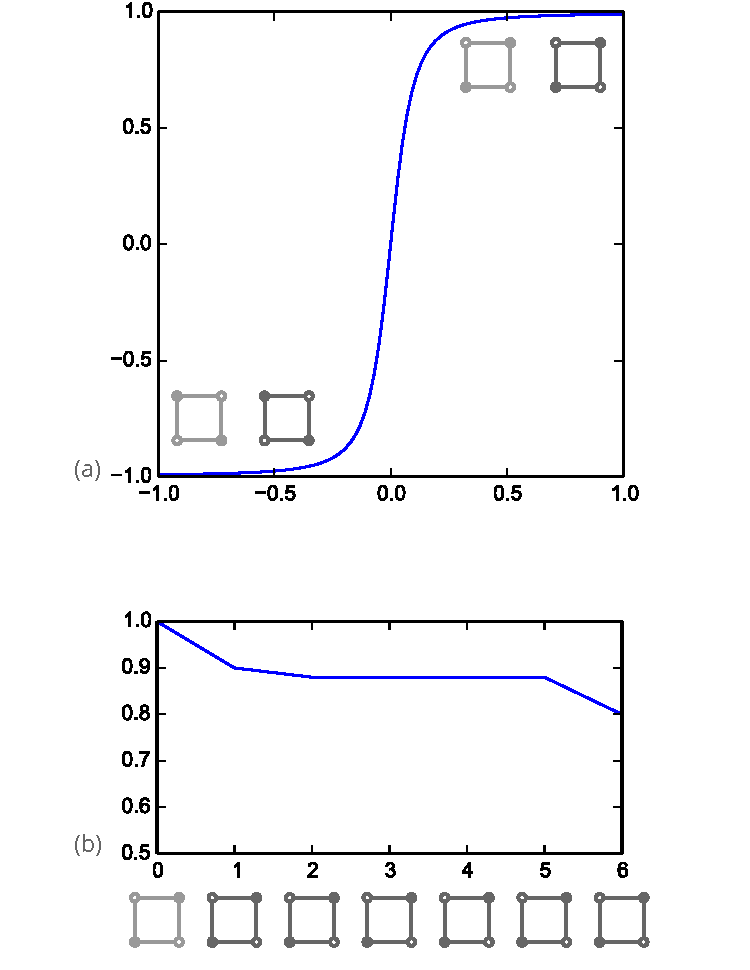
\includegraphics{qca_characterization}
  \caption{\ldots; TODO: frame of plots should be grey, not black}
  \label{fig:qca_characterization}
\end{figure}

At the time of this writing, the QCA idea is over twenty years old. Naturally,
the fundamental building blocks of QCA circuitry, such as the single cell
itself, the wire, and the majority gate, have been characterized, typically
numerically, but to a very limited extent also experimentally. Interestingly,
time-independent properties were investigated relatively briefly and arguably
not exhaustively. The bulk of the existing work soon focused on system dynamics,
building large scale computing architectures with the QCA paradigm, and on
specific potential experimental realizations. The characterization of
time-indepentend QCA properties yielded two main results. First, the cell-cell
response, that is, how the polarization of one cell responds to the polarization
of a neighbouring cell, was established to be non-linear and exhibit gain
\cite{lent1993quantum}. Therefore, even an only partially polarized cell would
fully polarize the cell next to it, Fig.~\ref{fig:qca_characterization}(a). Of
course, gain is highly desirable, if not essential, for building digital
circuits. It compensates any loss or imperfections and makes the scheme overall
robust. Not coincidentally, CMOS technology is built around the MOSFET
transistor with gain as one of its intrinsic properties. Second, lines of cells
were seen to be constantly polarized, Fig.~\ref{fig:qca_characterization}(b)
\cite{lent1993lines}. Thus, apart from few cells next to the driver cell, all
remaining cells in the line would be polarized with the same polarization, the
\emph{saturation} polarization. The \emph{saturation} polarization was observed
to be largely independent of the dirver cell's polarization, but solely
determined by the system's parameters such as the hopping $t$ and the Coulomb
energy $V_1$. For unfavourably chosen parameters the \emph{saturation}
polarization might be zero, but over a wide range of system parameters it was
shown to be close to perfect. For example, for large hopping $t$ the
\emph{saturation polarization} is expected to be zero. If $t$ is then decreased
passes a critical point $t_c$ a first order phase transition takes place, the
\emph{saturation} polarization becomes non-zero and in fact very quickly close
to perfect as $t$ is further decreased. In addition to the cell-cell response
and the analysis of a line of cells, larger QCA structures such as the majority
gate were reported to function correctly for a select set of parameters, but
were not analyzed in depth. Overall, the physical picture emerging from the
early time-independent calculations is of bistable cells readily snapping into
the correct fully polarized state throughout the whole device. It is a picture
where the QCA approach works almost perfectly over a presumably wide range of
parameters and it is the prevailing picture to this day. It is also quite wrong.

These early calculations of time-independent QCA properties concentrated almost
exclusively (with one exception \cite{tougaw1993bistable}) on the ground state
of the system. However, focusing solely on the ground state is not sufficient.
While the QCA approach is intended to be operated ``close to the ground state''
at least the first excited state is needed to obtain an estimate for the
operational temperature for these devices---a parameter of significant practical
interest. More subtly, what the QCA idea calls ``ground state'', ideally $P=-1$
or $P=1$, actually corresponds to multiple states, namely, one spin singlet and
three spin triplet states for $P=-1$ and $P=1$, respectively, in a single cell.
While these states can reasonably be expected to be near-degenerate, a thorough
study of QCA should still consider them. In more practical terms, QCA is
expected to operate at finite temperatures so simulating the devices at non-zero
temperature just makes sense. Similarly, the existing work on time-independent
QCA properties is not exhaustive in the exploration of other parameters. For
example, while the \emph{saturation} polarization's dependence on $V_1$ and $t$
is mapped out, concrete numerical values for these quantities are hard to come
by. In other cases the Coulomb scale $V_1$ is not indicated explicitly at all.
Cells are assumed to be charge-neutral, but the effects of non-charge-neutrality
is not investigated.  Different cell-cell distances are not discussed, nor what
system parameters should be chosen for optimal performance.

The exact numerical simulation of QCA systems is challenging and in fact
intractable for all but the smallest structures. Therefore, approximations are
necessary. In the literature on QCA two approximations are prevailing: The
intercellular Hartree approximation (ICHA) and the two-states-per-cell
approximation \cite{lent1993quantum} \cite{tougaw1996dynamic}. Most of the
studies of time-independent QCA properties employ the ICHA. Only the cell-cell
response is calculated with a ``full'' quantum mechanical model, where the
``full'' model is actually already the reduced Hilbert space of exactly two
electrons per cell. ICHA is a mean field scheme: The Hamiltonian of one cell is
solved exactly in the mean field of the polarizations of all the other cells.
More specifically, the cell-cell interaction term $H^{cc}_{kl}$ in
eq.~\eqref{eq:H_cell} is rewritten
\begin{equation}
\begin{split}
  \label{eq:H_kl_meanfield}
  H^{cc}_{kl} 
  %
  &=
  %
  \sum_{\substack{i \in k\\j \in l}} V_{ij} \left( n_i - q \right) \left( n_j - q \right) \\
  %
  &\sim
  %
  \sum_{\substack{i \in k\\j \in l}} V_{ij} 
       \left[ \frac{1}{2} 
              \left( n_i - q \right) \left( \left< n_j \right> - q \right)
              +
              \frac{1}{2}
              \left( \left< n_i \right> - q \right) \left( n_j - q \right)
       \right] \\
  %
  &\sim
  %
  \frac{1}{2} \sum_{i \in k} \left( n_i - q \right) \tilde{V}_i^l
       +
       \frac{1}{2} \sum_{j \in l} \left( n_j - q \right) \tilde{V}_j^k \, ,
\end{split}
\end{equation}
and the one-cell mean field Hamiltonian becomes
\begin{equation}
  \label{eq:H_meanfield}
  H_{mf} = H^c + \sum_i \left( n_i - q \right) \left( \sum_l \tilde{V}_i^l(\left<P_l\right>) \right) \, .
\end{equation}
Because the cell polarization is directly related to the occupancies of the
sites of the cell, we have $\tilde{V}_i^l = \tilde{V}_i^l(\left<P_l\right>)$.
Solving the one-cell Hamiltonian allows to compute to polarization $\left< P
\right>$ of the cell which in turn is used to set the mean field $\sum_l
\tilde{V}_i^l(\left<P_l\right>)$, with $\left<P_l\right> = \left<P\right>$,
originating from all other cells. The procedure is repeated until a
self-consistent cell polarization and thus self-consistent solution for
Eq.~\eqref{eq:H_meanfield} is found. By using, for example $n_i n_j \sim
\frac{1}{2} n_i \left< n_j \right> + \frac{1}{2} \left< n_i \right> n_j$, mean
field approximations neglect quantum fluctuations. Only at high dimensionality
can these fluctuations really average to zero and indeed mean field schemes can
be shown to become exact in the limit of infinite dimensionality \cite{Fehske}.
Conversely, for low dimensional systems fluctuations are more important and mean
field approximations are intuitively expected not to work very well. As
uncontrolled approximations the validity of mean field approaches needs to be
verified on a case by case basis. Because QCA is quasi-one-dimensional it is
arguably not well-suited for a mean field treatment. Even then a mean field
approximation might be appropriate as a first stab at the problem. However, the
infinite wire discussed above provides a simple example where ICHA already goes
wrong. We argued that due to entropy the infinite wire can only be ordered at
zero temperature. In contrast, a mean field approximiation will predict order up
to a finite critical temperature. ICHA was introduced in the very first QCA
paper. The approximation was never verified or complemented by more accurate
methods. It is rather remarkable that a large part of the existing work on QCA
characterization rests, directly or indirectly, on an approximation that can
reasonably be expected to give wrong results. And indeed, in the context of the
dynamic properties of QCA it has been known for a long time that ICHA gives
qualitatively wrong results \cite{toth2001role}. Much more recently, it has been
shown very explicitly that even for the single cell-cell response ICHA
introduces artifacts that are clearly non-physical
\cite{taucer2012consequences}.
% TODO: more detail, why do we expect the mean field approach to give a finite
% critical temperature for the infinite wire. Can I use an analogy to the
% three-dimensional classical Ising model --- where mean-field works pretty
% well?
% TODO: better citation for the fact that mean field becomes exact in infinite
% dimensions

For the calculation of time-dependent properties the two-states-per-cell
approximation is typically used, precisely because it was realized that ICHA
does give wrong results, for example for the switching behaviour of some
majority gate structures. Perplexingly, in the literature the two-state
approximation is motivated and justified by the ICHA picture
\cite{tougaw1996dynamic}. Starting from the observation that wires are polarized
with a \emph{saturation} polarization (in ICHA calculations), a cell is
represented by two basis states, corresponding to $P = P_{sat}$ and $P = -
P_{sat}$. In a loose sense, the two-states-per-cell model thus comes from a
picture of how we would like QCA to work: Perfectly bistable, interacting cells.
The approximation has been verified to the extent that it was shown that the
ground state of the full quantum mechanical model can be represented nearly
perfectly by the two-state basis, but only for one cell and for one particular
set of system parameters. In a more rigorous treatment it should be possible to
clearly derive the two-state model as the correct emerging low-energy
Hamiltonian from the original extended Hubbard model. Such a derivation would
also work out the parameter regime where the effective two-state Hamiltonian is
valid. We will attempt it in due course. In contrast to ICHA the
two-states-per-cell approximation retains inter-cell entanglement and therefore
yields more correct results, not only for dynamics, but also for
time-independent properties. As the price the two-state model scales
exponentially, whereas ICHA scales linearly in system size.  Therefore, even
with the two-state approximation only relatively small QCA devices are
computationaly feasible. As a last note, the two-state model is clearly very
similar to a transverse field quantum Ising model, where the two polarization
states correspond to a pseudo spin and the hopping is like a transverse field,
flipping the cell polarizations.


\section{Exact diagonalization}

We use the exact diagonalization numerical method \cite{Fehske} to simulate QCA
systems described by the Hamiltonian \eqref{eq:H_QCA}. In principle, exact
diagonalization is a straightforward method: For a chosen basis the matrix of
the Hamiltonian is constructed explicitly and then diagonalized, yielding the
eigenenergies and eigenstates of the system. With that we know everything about
the system and can calculate observables of interest. The problem is that memory
consumption scales as $N_s^2$ and the computational cost roughly as $N_s^3$,
where $N_s$ is the size of the state space; and the number of states scales
exponentially with system size, $N_s = 4^{N_d} = 256^{N_c}$. $N_d$ denotes the
number of dots and $N_c$ the number of cells. As an example, to store the full
Hamiltonian matrix of a two cell QCA system requires 3GB of memory, to store the
Hamiltonian matrix of a three cell system already requires 2000TB. That's
clearly not feasible on any available computer. As a side note, we cannot employ
projective algorithms like Lanczos \cite{Fehske}, because we are interested in
finite temperatures and therefore need the full energy spectrum. Typically,
projective schemes are only useful to calculate the ground state or the few
lowest energy states. 

\newcommand{\ket}[1]{\left|#1\right>}
\newcommand{\bra}[1]{\left<#1\right|}
%
To decrease the memory requirements and computational cost of
exact diagonalization symmetries must be exploited. The Hamiltonian matrix is
actually quite sparse---most entries are zero. By using symmetries and a
suitable basis the Hamiltonian matrix can be brought into block diagonal form
and then only those much smaller blocks need to be diagonalized. Our QCA system
is symmetric with respect to the total particle number $\hat{N} = \sum_i
\hat{n}_{i\uparrow} + \hat{n}_{i\downarrow}$ and the total spin $\hat{S} =
\sum_i \hat{n}_{i\uparrow} - \hat{n}_{i\downarrow}$, i.e.\ $[\hat{N},\hat{H}]_-
= [\hat{S},\hat{H}]_- = 0$. If we now use basis states which are eigenstates of
the symmetry operators, $\ket{n,s,l}$, with
%
\begin{equation}
\begin{split}
  \hat{N} \ket{n,s,l} &= n \ket{n,s,l} \, , \\
  \hat{S} \ket{n,s,l} &= s \ket{n,s,l} \, ,
\end{split}
\end{equation}
%
then we have
%
\begin{equation}
\begin{split}
  \bra{n^{\prime},s^{\prime},l^{\prime}} [\hat{N},\hat{H}]_- \ket{|n,s,l} = 
  (n^{\prime} - n) \bra{n^{\prime},s^{\prime},l^{\prime}} \hat{H} \ket{n,s,l}
  \stackrel{!}{=} 0 \\
  \bra{n^{\prime},s^{\prime},l^{\prime}} [\hat{S},\hat{H}]_- \ket{n,s,l} = 
  (s^{\prime} - s) \bra{n^{\prime},s^{\prime},l^{\prime}} \hat{H} \ket{n,s,l}
  \stackrel{!}{=} 0
\end{split}
\end{equation}
%
and therefore
%
\begin{equation}
  \bra{n^{\prime},s^{\prime},l^{\prime}} \hat{H} \ket{n,s,l} = 0 \qquad
  \textrm{for } n \ne n^{\prime} \textrm{ or } s \ne s^{\prime} \, .
\end{equation}
%
Consequently, by ordering basis states by the symmetry operators' eigenvalues
the Hamiltonian matrix becomes block diagonal, where the blocks are labelled by
$n$ and $s$. The blocks can be constructed and diagonalized separately and all
observables can then be calculated block-wise as well, hence vastly reducing
memory requirements and computational time. In our implementation, however, we
do keep all blocks in memory simultaneously. This still yields considerably
reduced memory usage and the same speedup in computational time. For the QCA system
the single largest block is the spin zero sector at half-filling. Its size is
%
\begin{equation}
  N_s^{\prime} = \binom{N_d}{\frac{1}{2} N_d}^2 \, .
\end{equation}
%
This corresponds to memory requirements of 180MB for two cells and 5400GB for
three cells. Thus, although this is a considerable improvement for the two cell
system (not least in computational time), the three cell system still remains
unreachable with conventional computer hardware. To access larger systems we
need to introduce approximations, which we will pursue in detail and with great
care in the following chapter.

Computational physics is, true to its name, to considerable extent concerned
with writing computer code. If ingenious algorithms which bring sophisticated
physical problems to the computer are the art that excites the computational
physicist's intellect, then writing good computer code is the craft. It is a
curious fact that traditionally in computational condensed matter physics little
weight has been put on coding techniques, collaboration on the code level, and
the code itself. This not only frustrates the newcomer to the field, for it is a
long way from a formally stated algorithm to a correct and efficient
implementation, but also poses a more fundamental problem to science in a time
when computing has long become an essential part of it. Scientific results
obtained from sophisticated numerical algorithms can be difficult to verify and
reproduce without an openly available implementation of those algorithms. But
verification and reproducibility are core assets of the scientific process.
Fortunately, the culture is slowly changing. In computational condensed matter
physics, the ALPS and Abinit projects provide open implementations of a variety
of commonly used methods and algorithms \cite{bauer2011alps}
\cite{gonze2009abinit}. In the wider scientific community, IPython is a shining
example of building a powerful computational tool collaboratively, with a huge
impact across disciplines \cite{perez2007ipython}.

Our QCA exact diagonalization implementation is written in C++ and uses the
excellent Eigen linear algebra library \cite{eigen}. Matrices are stored in
sparse representation, except for the block-wise diagonalization itself,
performed by Eigen, where we use dense matrices. The basis states can be
filtered and sorted, e.g.\ to truncate the Hilbert space to a specific charge
sector and to exploit symmetries. We do not build the Hamiltonian matrix
directly, but instead construct creation and annihilation operator matrices.
Therefore, operators such as the Hamiltonian and the polarization can be
expressed in an intuitive, almost mathematical notation. We employ the curiously
recurring template pattern to achieve simple static polymorphism, avoiding the
overhead of runtime polymorphism \cite{andrei2001modern}. In less abstract
terms, this allows us to reuse code, for example the Hamiltonian, for the
conceptually similar, but physically quite different various QCA models which we
are going to introduce in detail in the next chapter. Our C++ code cannot be
executed directly, but is instead compiled as an extension module for the Python
language, via the Boost library's Boost.Python \cite{boost}. We also use the
unit testing framework from the Boost library. In our experience, making the C++
code available in Python provides enormous benefits. With Python data input,
output and storage becomes a breeze, especially compared to the chore these
tasks are in pure C++. Python makes it easy to script and distribute (i.e.\
simply parallelize) simulation runs, and, being well established in the
scientific community, comes with extensive libraries for data analysis and
plotting, e.g.\ SciPy and Matplotlib \cite{scipy} \cite{hunter2007matplotlib}.
Consequently, the integration with Python facilitates quickly trying out new
ideas, implementing new features and more fluid data analysis. The advent of the
fantastic IPython notebook ties all of these pieces together in a consistent,
productive and highly enjoyable workflow \cite{perez2007ipython}. The IPython
notebook is also an apt format for effectively communicating results with
colleagues. The disadvantages of the Python integration are the additional
dependencies, although both Python and Boost are commonly available on any
number of platforms these days, and the more involved (and hence error-prone)
build process. We have written a small Python library to support our data
storage and organization needs. The library facilitates storing and retrieving
data in standard file formats and allows to define and run ``numerical
experiments,'' which can be distributed across multiple computers. Both the QCA
exact diagonalization code and the Python library are available under an open
license on GitHub \cite{githubqca} \cite{githubcoma}.




















% previous work / early papers
%
% Compensation charge is mentioned, but not explicitly written down in the
% equation. All cells are charge neutral.
%
% They only look at spin-singlets, i.e. 16 state cell. They say, in a rather
% vague manner, that results for parallel spins exhibit "nearly identical
% behaviour".
%
% This is actually not correct: The following paper explicitly mentions the
% singlet-triplet splitting: "Lines of interacting quantumdot cells: A binary
% wire" Craig S. Lent and P. Douglas Tougaw, J. Appl. Phys. 74, 6227 (1993)
% 
% Almost all calculations are for the ground state. One of the early papers
% looks at the cell-cell response as a function of temperature.
%
% They do calculations for a ranges of parameters, notably $t$ is varied. Still,
% overall parameters are pretty vague. They use an "experimentally reasonable"
% model of circular quantum dots with a given diameter and given spacing; and
% given inter-cell spacing. But the concrete (derived) Coulomb energy used is
% not explicitly stated, as far as I can tell.
%
% Only the one-cell cell-cell response is calculated exactly (16 state basis).
% All other calculations are ICHA. ICHA is never verified.
%
% They investigate a wire: Wires tend to a constant saturation polarization,
% which depends on the system parameters and can be zero (wire "fails"). All of
% this is with the ICHA approximation. The picture of nicely constantly
% polarized wires (with $P_{sat}$) emerges. They look at $P_{sat}$ in terms of
% the hopping $t$ and the inter-cell distance.
%
% They explain: The ground state is two degenerate states with P=-1 and P=+1.
% ---This is wrong. The ground state without external perturbations is a
% superposition of the P=-1 and P=+1 states (in a rough approximation) with P=0.
% The very notion of "bistable" cells is a little bit problematic, in my
% opinion. (Even though I used it myself in the introduction above. Maybe I
% should avoid the word bistable...).
%
% They argue that ICHA is only good for the ground state (1996 JApplPhys paper).
% To argue against that I need to show ground state calculations, T=0, that show
% ICHA does not give the right result. I should also argue that ground state
% calculations are not enough. 
%
% I need good arguments to explain why ICHA needs proper verification, why there
% is reason to be suspicious about the approach, even for the ground state.
%
% Maybe I could also explicitly address why even only 16 states for the single
% cell is not good enough. (I believe that, for example, for the two cell system
% the ground state is not singlet, though I would have to verify that.)
%
% They calculate dynamics of three cells exactly with the 16-state-per-cell
% basis (1996 JApplPhys paper).
%
% Two state basis is introduced empirically, motivated by the "bistable" cell with
% a saturation polarization $\pm P_{sat}$ from ICHA calculations (specifically
% for the binary wire). To verify the two-state basis, they calculate the
% overlap with the 16-state basis for a single (active) cell system, for some
% unspecified set of system parameters. (They do this for ground state and first
% excited state.) They find that the two selected basis states almost complete
% span the Hilbert space in this case. They do a time-dependent calculation for
% a three-cell wire and compare this with a calculation using the 16-state
% basis. All of this is done for only one set of parameters (which are not
% explicitly stated.) They map to the Ising model. They do dynamics (with the
% two-state basis) for a majority gate, a eight-cell wire and a semi-infinite
% wire.





% TODO:
% Emphasize somewhere that by using the Hubbard model our calculations and results
% might not be applicable to QCA implementations that are decidedly not
% well-described by Hubbard physics.
%
% Maybe explicitly mention quasiadiabatic switching.
% 
% Rethink / rewrite clocking: How the gate voltage changes the barrier.
